\documentclass[11pt]{article}
\usepackage[left=3.5cm,right=3.5cm,top=2.5cm,bottom=2.5cm]{geometry}
%\usepackage[spanish]{babel}

\usepackage{amsmath,amsfonts,amsthm}
\usepackage{enumitem,mathtools,graphicx}
\setenumerate[0]{label=(\alph*)}

\newtheorem{definition}{Definición}
\newtheorem{exercise}{Ejercicio}
\newtheorem*{sol}{Solución}
\newtheorem*{theorem}{Teorema}

\newcommand\N{\mathbb N}
\newcommand\R{\mathbb R}

\title{Análisis numérico para ecuaciones diferenciales \\
Tarea 1 - Introducción a los métodos de un paso}
\author{Jorge Alfredo Álvarez Contreras}

\begin{document}
\maketitle

\begin{definition}[Método de Euler]
  Dado un problema de valores iniciales
  \begin{equation}\label{eq:pvi}
    \left\{
      \begin{aligned}
        y'(t) &= f(t,y) \\
        y(0) &= y_0
      \end{aligned}
    \right.
  \end{equation}
\end{definition}

\begin{exercise}
  Demuestre que el método de Euler es cero-estable cuando es aplicado
  al problema de valores iniciales $y'=-1/y^{2}$, $y(0)=y_0$, donde
  $y_0\in[a,b]$ para $0<a<b$.
\end{exercise}

\begin{sol}
  La situación del problema está dada por el PVI \eqref{eq:pvi},
  donde $f(t,y)=f(y)=-\frac{1}{y^{2}}$.
  Fíjese $N\geq 1$ tan grande como se quiera,
  de modo que, al menos, $a\geq 1 / N$. Entonces $f=f(y)$ es de
  Lipschitz en $[1 / N,\infty)$, ya que para $y_1,y_2\geq 1 / N$ se
  tiene $N\geq \frac{1}{y_1}$ y $N\geq \frac{1}{y_2}$, de modo que
  \begin{align}
    |f(y_2)-f(y_1)|
    &= \left|-\frac{1}{y_2^{2}}+\frac{1}{y_1^{2}}\right| \\
    &= \left|\frac{y_2^{2}-y_1^{2}}{y_1^{2}y_2^{2}}\right| \\
    &= \frac{y_2+y_1}{y_1^{2}y_2^{2}} |y_2-y_1| \\
    &=
    \left(
      \frac{1}{y_1^{2}y_2}
      +
      \frac{1}{y_1y_2^{2}} 
    \right)
    |y_2-y_1| \\
    &\leq 2N^{3} |y_2-y_1|
  .\end{align}

  Por el teorema de estabilidad cero, esto implica que, para
  intervalos de tiempo $[0,T]$ pequeños (lo suficientemente pequeños
  como para que $y(t)$ no disminuya por debajo de $1 / N$)
  entonces el método de Euler es cero-estable.
\end{sol}

\begin{exercise}
  Implemente en Python los métodos de Euler y Heun. Posteriormente
  utilice estos métodos para resolver el PVI
  \begin{equation}
    \left\{
      \begin{aligned}
        y' &= yt^{3} - 3y / 2, \\
        y(0) &= 1,
      \end{aligned}
    \right.
  \end{equation}
  con $h=0.2$ en $t\in [0,2]$. Elabore dos gráficas, una con la
  aproximación obtenida contra la solución analítica y otra del error
  puntual.
\end{exercise}
\begin{sol}
  \begin{figure}[ht]
    \centering
    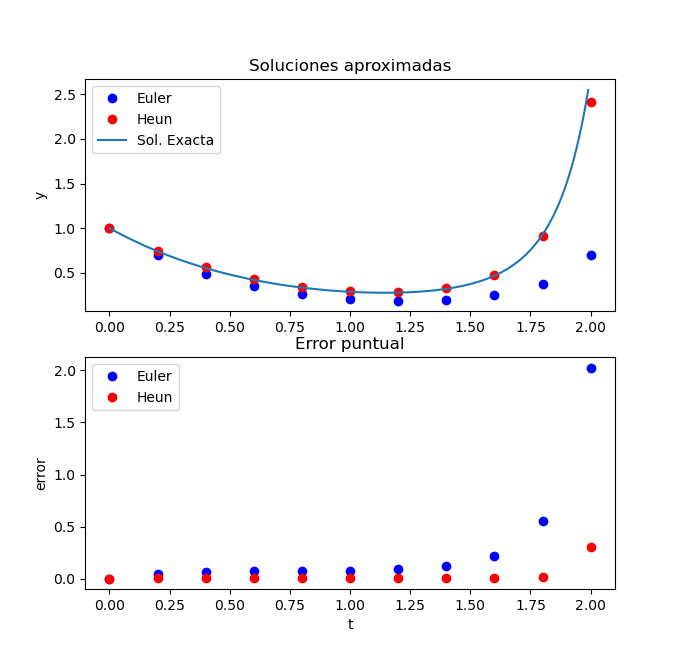
\includegraphics[width=0.5\textwidth]{img/jaac_tarea1_ejercicio2}
    \caption{Resultados del ejercicio 2: soluciones aproximadas para
      $y'(t)=yt^{3}-\frac{3y}{2}$.
      La solución exacta es $y(t)=\exp(t^{4} / 4 - 3t / 2)$.}
    \label{fig:exe_1}
  \end{figure}
\end{sol}

\begin{exercise}
  Adapte los programas de Python que elaboró en el ejercicio anterior
  para resolver sistemas de ecuaciones. Utilice dichos programas para
  resolver numéricamente el oscilador de Van der Pol:
  \begin{equation}
    y'' + (y^{2}-1)y' + y = 0
  .\end{equation}
  Grafique las órbitas con $y(0)=0$, $y'(0)=1$ y con $y(0)=-2$,
  $y'(0)=3$. Utilice el mismo valor de $h$ para ambos métodos y
  presente dichas órbitas en una figura distinta para cada método.
\end{exercise}
\begin{sol}
  \leavevmode
  \begin{figure}[hb]
    \centering
    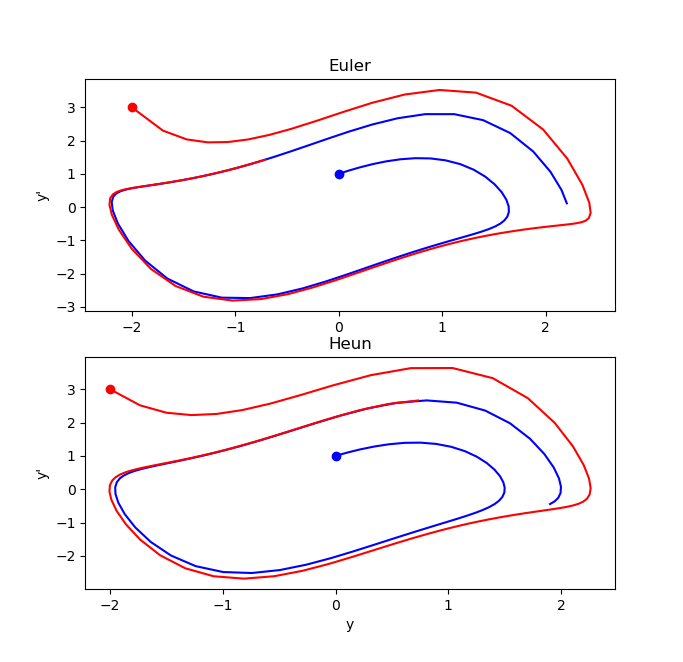
\includegraphics[width=0.5\textwidth]{img/jaac_tarea1_ejercicio3}
    \caption{Resultados del ejercicio 3: soluciones aproximadas para
      el oscilador de Van der Pol: $y'' + (y^{2}-1)y' + y = 0$}
    \label{fig:exe_2}
  \end{figure}
\end{sol}

\begin{exercise}
  Calcule el error de truncamiento local y el orden del método
  trapezoidal.
\end{exercise}
\begin{sol}
  El método trapezoidal está definido como
  \begin{equation}
    u_{n+1} = u_n + \frac{h}{2}[f_n + f_{n+1}]
  \end{equation}
  con $u_0=y_0$.
  El error de truncamiento local $\tau_{n+1}$ es el cociente
  $\epsilon_{n+1} / h$, donde
  \begin{equation}
    y_{n+1} = y_n + \frac{h}{2}[f(t_n,y_n)+f(t_{n+1},y_{n+1})] +
    \epsilon_{n+1}
  .\end{equation}
  Expandiendo en serie de Taylor:
  \begin{equation}\label{eq:taylor_trapezoidal}
    \begin{split}
    &\hspace{-5mm}
    y_{n}+hy'_n+\frac{h^{2}}{2}y''_n+\frac{h^{3}}{3!}y'''(\xi)
    \\
    &=
    y_n
    +
    \frac{h}{2} \left[
      2y'_n + h Df(t_n,y_n)((1,y'_n))
      + \frac{h^{2}}{2} D^{2}f(z)((1,y'_n),(1,y'_n))
    \right]
    + \epsilon_{n+1},
    \end{split}
  \end{equation}
  donde $\xi\in(t_n,t_{n+1})$ y $z\in\R^{2}$ es un vector en el
  segmento de recta que conecta a los puntos $(t_n,y_n)$ y
  $(t_{n+1},y_{n+1})$. Notando que
  \begin{align}
    Df(t_n,y_n)((1,y'_n))
    &= \frac{\partial f}{\partial t}(t_n,y_n)
    + \frac{\partial f}{\partial y}(t_n,y_n)y'_n \\
    &= y''_n
  \end{align}
  la expresión \eqref{eq:taylor_trapezoidal} se simplifica a
  \begin{equation}
    \frac{h^{3}}{3!}y'''(\xi)
    =
    \frac{h^{3}}{4} D^{2}f(z)((1,y'_n),(1,y'_n))
    + \epsilon_{n+1},
  .\end{equation}
  Luego,
  \begin{equation}
    \tau_{n+1}(h)
    =
    \frac{\epsilon_{n+1}}{h}
    =
    \frac{h^{2}}{2}
    \left(
      \frac{1}{3}y'''(\xi)
      -
      \frac{1}{2}D^{2}f(z)((1,y'_n),(1,y'_n))
    \right)
    = O(h^{2})
  .\end{equation}
  Si, por ejemplo, tenemos cotas
  $|y'''|\leq M_1$, $|y'|\leq M_2$ en $I$ y
  $\|D^{2}f\|\leq M_3$ en el segmento de recta que conecta a
  $(t_n,y_n)$ con $(t_{n+1},y_{n+1})$, entonces
  \begin{equation}
    |\tau_{n+1}(h)|\leq \frac{h^{2}}{2}
    \left(
      \frac{M_1}{3} + \frac{(1+M_2^{2})M_3}{2}
    \right)
  \end{equation}
  para todo $n$, así que tenemos la siguiente cota para el error de
  truncamiento global:
  \begin{equation}
    \tau(h)
    \leq
    \left( \frac{M_1}{3} + \frac{(1+M_2^{2})M_3}{2}  \right)
    \frac{h^{2}}{2}
  .\end{equation}
\end{sol}

\begin{exercise}
  Considere el método
  \begin{equation}
    u_{n+1} = u_n + h[af_n + bf(t_n+\alpha h,u_n+\beta h f_n)]
  \end{equation}
  donde $a,b,\alpha,\beta$ son parámetros reales.
  \begin{enumerate}
    \item
      Establezca condiciones sobre los parámetros $a,b,\alpha,\beta$ 
      para garantizar que el método es de primer orden.
    \item
      Pruebe que existe una combinación de estos parámetros tal que el
      método es de segundo orden. ¿Existe alguna combinación de las
      constantes de tal manera que el orden es mayor a $2$?
  \end{enumerate}
\end{exercise}
\begin{sol}
  \begin{enumerate}
    \item
      En los puntos $y_n$, $y_{n+1}$, tenemos
      \begin{equation}\label{eq:sin_expandir}
        y_{n+1}
        = y_{n} + h[ay'_n + bf(t_n + \alpha h, y_n + \beta h y'_n)] +
        \epsilon_{n+1}
      .\end{equation}
      Expandiendo en serie de Taylor hasta primer orden en $h$,
      tenemos
      \begin{equation}
        y_n + hy'_{n} + O(h^{2})
        = y_{n} + h[ay'_n + b f(t_n,y_n) + O(h)] +
        \epsilon_{n+1}
      \end{equation}
      notando que $f(t_n,y_n)=y'_n$, esto es
      \begin{equation}
        y_n + hy'_{n} + O(h^{2})
        = y_{n} + h(a+b)y'_n + O(h^{2}) +
        \epsilon_{n+1}
      .\end{equation}
      Si se cumple $a+b=1$, los primeros dos términos de cada lado se
      cancelan y tenemos $\epsilon_{n+1} = O(h^{2})$, por lo cual
      \begin{equation}
        \tau_{n+1}(h) = \frac{\epsilon_{n+1}}{h} = O(h)
      .\end{equation}
    \item
      Volviendo a expandir la expresión \eqref{eq:sin_expandir} en
      serie de Taylor, pero ahora hasta orden $2$ en $h$, obtenemos
      \begin{equation}
        \begin{split}
          &\hspace{-5mm}
          y_n + hy'_{n} + \frac{h^{2}}{2}y''_n + O(h^{3}) \\
          &= y_{n}
          + h[
          ay'_n + b f(t_n,y_n) + bh Df(t_n,y_n)((\alpha, \beta y'_n))
          + O(h^{2})]
          + \epsilon_{n+1}
        \end{split}
      \end{equation}
      De nuevo, notemos que $f(t_n,y_n)=y'_n$, así que
      \begin{equation}
        \begin{split}
          &\hspace{-5mm}
          y_n + hy'_{n} + \frac{h^{2}}{2}y''_n + O(h^{3}) \\
          &= y_{n}
          + h(a+b)y'_n
          + bh^{2} Df(t_n,y_n)((\alpha, \beta y'_n))
          + O(h^{3})
          + \epsilon_{n+1}
        \end{split}
      \end{equation}
      Como vimos antes, para que el método sea de orden $1$ (al
      menos), debemos pedir que $a+b=1$, con lo cual se cancelan los
      primeros dos términos de cada lado.
      Además, si $\alpha=\beta$, entonces podemos sacar $\alpha$ del
      término de orden $2$, el cual se convierte en un múltiplo de
      $Df(t_n,y_n)((1,y'_n))=y''_n$, es decir:
      \begin{equation}
          y_n + hy'_{n} + \frac{h^{2}}{2}y''_n + O(h^{3})
          = y_{n}
          + hy'_n
          + \alpha bh^{2} y''_n
          + O(h^{3})
          + \epsilon_{n+1}.
      \end{equation}
      Los primeros dos términos se cancelan. Finalmente, si requerimos
      que $\alpha b=\frac{1}{2}$, entonces el tercer término también
      se cancela, con lo cual obtenemos $\epsilon_{n+1}=O(h^{3})$.
      Luego,
      \begin{equation}
        \tau_{n+1}(h) = \frac{\epsilon_{n+1}}{h} = O(h^{2})
      .\end{equation}
      En resumen, para que el método sea de orden $2$, las condiciones
      son $a+b=1$ y $\alpha=\beta=\frac{1}{2b}$.
    \item
    No se pueden elegir constantes para que el método sea de orden
    $3$. En efecto, después de imponer las condiciones para que el
    método sea de orden $2$, tenemos
    \begin{equation}\label{eq:nosepuede}
      \frac{h^{3}}{3!}y'''_n + O(h^{4})
      = b\frac{h^{3}}{2}D^{2}f(t_n,y_n)((1,y'_n),(1,y'_n))
      + \epsilon_{n+1}
      + O(h^{4})
    .\end{equation}
    Sin embargo, el término $y'''_n$ no se puede cancelar con nada del
    lado derecho, ya que, aunque $y''_n = Df(t_n,y_n)((1,y'_n))$,
    tenemos
    \begin{equation}
      y'''_n = D^{2}f(t_n,y_n)((1,y'_n),(1,y'_n)) +
      Df(t_n,y_n)(0,y''_n)
    \end{equation}
    y este último término, que incluye $y''_n$, no se puede cancelar
    con ninguna elección de $b$.
    \iffalse
    La elección que más simplifica la
    expresión \eqref{eq:nosepuede} es tomar $b=\frac{1}{3}$, de modo
    que
    \begin{equation}
      \frac{h^{3}}{3!}y'''_n + O(h^{4})
      = \frac{h^{3}}{3!}D^{2}f(t_n,y_n)((1,y'_n),(1,y'_n))
      + \epsilon_{n+1}
      + O(h^{4})
    \end{equation}
    y entonces
    \begin{equation}
      \epsilon_{n+1}
      =
      \frac{h^{3}}{3!}Df(t_n,y_n)(0,y''_n)
      + O(h^{4})
    \end{equation}
    \fi
  \end{enumerate}
\end{sol}

\begin{exercise}
  Considere el método de un paso dado por
  \begin{equation}
    u_{n+1} = u_n + h \left[
      f_n + \frac{h}{2}g \left(
        t_n + \frac{1}{3}h,
        u_n + \frac{1}{3}hf_n
      \right)
    \right]
  ,\end{equation}
  donde $g=f_t+ff_y$. Muestre que el método es de orden $3$.
\end{exercise}
\begin{sol}
  El error residual $\epsilon_{n+1}$ satisface
  \begin{equation}
    y_{n+1} = y_n + h \left[
      y'_n + \frac{h}{2}g \left(
        t_n + \frac{1}{3}h,
        y_n + \frac{1}{3}hy'_n
      \right)
    \right]
    + \epsilon_{n+1}
  .\end{equation}
  Expandiendo el lado izquierdo en serie de Taylor hasta orden $3$ en
  $h$, tenemos
  \begin{equation}
    y_n + hy'_n + \frac{h^{2}}{2}y''_n + \frac{h^{3}}{3!}y'''_n +
    O(h^{4})
    = y_n + h \left[
      y'_n + \frac{h}{2}g \left(
        t_n + \frac{1}{3}h,
        y_n + \frac{1}{3}hy'_n
      \right)
    \right]
    + \epsilon_{n+1}
  \end{equation}
  con lo cual podemos cancelar los primeros dos términos y obtener
  \begin{equation}
    \frac{h^{2}}{2}y''_n + \frac{h^{3}}{3!}y'''_n +
    O(h^{4})
    = \frac{h^{2}}{2}g \left(
        t_n + \frac{1}{3}h,
        y_n + \frac{1}{3}hy'_n
      \right)
    + \epsilon_{n+1}
  \end{equation}
  Ahora tenemos
  \begin{equation}\label{eq:aquisisepudo}
    \frac{h^{2}}{2}y''_n + \frac{h^{3}}{3!}y'''_n +
    O(h^{4})
    =
    \frac{h^{2}}{2}g(t_n,y_n)
    +
    \frac{h^{3}}{3!}Dg(t_n,y_n)(1,y'_n) + O(h^{4})
    + \epsilon_{n+1}.
  \end{equation}
  Derivando ambos lados de la igualdad $y'(t)=f(t,y(t))$, tenemos
  \begin{align}
    y''(t)
    &= f_t(t,y(t))+f(t,y(t))f_y(t,y(t)) \\
    &= f_t(t,y(t))+y'(t)f_y(t,y(t)) \\
    &= g(t,y(t)),
    \\
    y'''(t)
    &= g_t(t,y(t)) + g_y(t,y(t)) y'(t) \\
    &= Dg(t,y(t))(1,y'(t)).
  \end{align}
  Por lo tanto, los primeros dos términos de cada lado de
  \eqref{eq:aquisisepudo} se cancelan y obtenemos
  $\epsilon_{n+1}=O(h^{4})$, de modo que
  \begin{equation}
    \tau _{n+1}(h) = \frac{\epsilon_{n+1}}{h} = O(h^{3})
  ,\end{equation}
  como se quería.
\end{sol}

\begin{exercise}
  Demuestre el teorema de convergencia 11.2 del libro de Quarteroni.
\end{exercise}
\begin{theorem}[Convergencia. p. 487]
  Si, en el método de un paso
  \begin{equation*}
    u_{n+1} = u_n + h\Phi(t_n,u_n,f_n;h),
    \quad
    0\leq n\leq N_h-1,
    \quad
    u_0=y_0
    \tag{11.11}
  ,\end{equation*}
  la función de incremento $\Phi$ es de Lipschitz en su segunda
  entrada, con constante de Lipschitz $\Lambda$ independiente de $h$ 
  y de los nodos $t_j\in[t_0,t_0+T]$, entonces se cumple
  \begin{equation*}
    |y_n-u_n|\leq (|y_0-u_0|+nh\tau(h))e^{nh\Lambda},
    \quad
    1\leq n\leq N_h
    \tag{11.20}
  .\end{equation*}
  Por lo tanto, si se satisface la hipótesis de consistencia
  \begin{equation*}
    \lim_{h\to 0} \Phi(t_n,y_n,f(t_n,y_n);h) = f(t_n,y_n),
    \quad
    \forall t_n\geq t_0
    \tag{11.13}
  \end{equation*}
  y $|y_0-u_0|\to 0$ cuando $h\to 0$, entonces el método es
  convergente. Más aún, si $|y_0-u_0|=O(h^p)$ y el método tiene orden
  $p$, entonces también tiene orden de convergencia $p$.
\end{theorem}

\end{document}
